% !TEX root = report.tex

\section{Processing Pipeline}
\label{sec:processing_architecture}

At a high level, both of our models cast Wi-Fi HAR as the classification of
Doppler-spectrogram images and share the \emph{same} data front-end; they differ
only in \emph{how} the representation is learned. \fig{fig:pipeline} sketches the
two chains. Common to both, the raw CSI Doppler traces are cut into fixed-size
windows of shape $1\times340\times100$ (one antenna at a time), which become the
network inputs (\secref{sec:model}). From here the pipeline forks:
\begin{itemize}
  \item the \textbf{baseline chain} (M.~Carraro) feeds each window to an
  Inception-style CNN trained end-to-end with cross-entropy, and reads the
  activity off the softmax output;
  \item the \textbf{contrastive chain} (F.~Vezzani) first applies
  domain-randomization augmentations to build two views of each window, pre-trains
  a deeper batch-normalized encoder with a Supervised Contrastive loss, then
  \emph{freezes} the encoder and fits a linear probe on the resulting features.
\end{itemize}
Both chains are trained on a single environment ($S1$) and evaluated under the
same cross-domain protocol (test on the unseen $S2$--$S7$), so that the two
learning strategies can be compared on equal footing against the reference SHARP
system~\cite{sharp}. The learning frameworks behind the two blocks are detailed
in \secref{sec:learning_framework}.

\begin{figure}[t]
  \centering
  \resizebox{\columnwidth}{!}{%
  \begin{tikzpicture}[
    font=\footnotesize,
    >={Stealth[length=2mm]},
    box/.style={rectangle, rounded corners=2pt, draw=black!70, thick,
                align=center, inner sep=4pt},
    data/.style={box, fill=green!12, text width=42mm},
    base/.style={box, fill=blue!12, text width=36mm},
    cont/.style={box, fill=yellow!20, text width=44mm},
    eval/.style={box, fill=orange!22, text width=46mm},
    arr/.style={->, thick, black!65},
  ]
    \node[data] (win) at (0,0)
      {Doppler windows\\$1\times340\times100$ (per antenna)};
    \node[base] (bcnn) at (-3.6,-2.6)
      {\textbf{Baseline (Carraro)}\\Inception CNN $+$ softmax};
    \node[cont] (enc) at (3.6,-2.6)
      {\textbf{Contrastive (Vezzani)}\\aug.\ $\to$ SupCon encoder\\$\to$ freeze $\to$ linear probe};
    \node[eval] (ev) at (0,-5.2)
      {Cross-domain evaluation\\train $S1$ / test $S2$--$S7$};

    \draw[arr] (win.south) -- (bcnn.north);
    \draw[arr] (win.south) -- (enc.north);
    \draw[arr] (bcnn.south) |- (ev.west);
    \draw[arr] (enc.south) |- (ev.east);
  \end{tikzpicture}%
  }
  \caption{High-level processing pipeline. A shared front-end turns CSI traces
  into Doppler windows; the baseline chain (M.~Carraro) classifies them directly,
  while the contrastive chain (F.~Vezzani) learns an environment-invariant
  representation before a linear probe. Both are assessed with the same
  cross-domain protocol.}
  \label{fig:pipeline}
\end{figure}

\section{Signals and Features}
\label{sec:model}
\emph{(Dataset pipeline implemented by M.~Carraro.)}

\begin{figure*}[t]
  \centering
  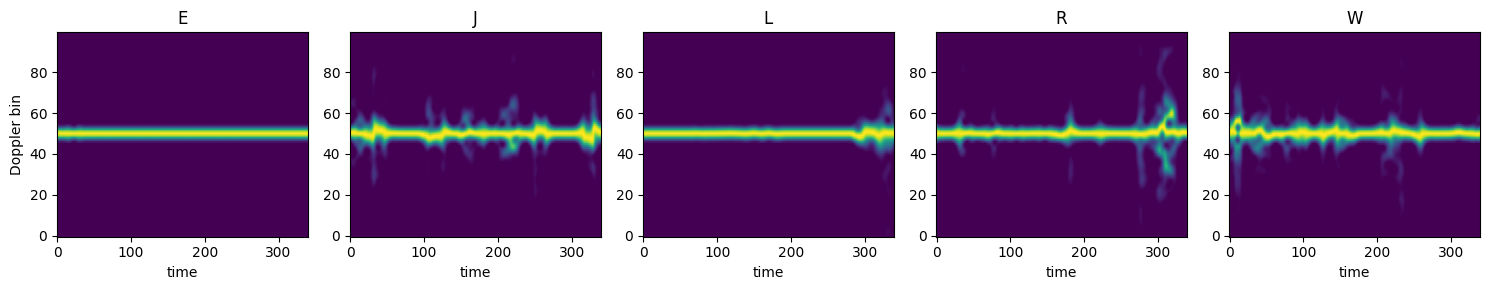
\includegraphics[width=\textwidth]{doppler_activities.png}
  \caption{One example Doppler-spectrogram window per activity (input to the
  network, transposed for readability: rows are the $100$ Doppler-velocity bins,
  columns are the $340$ time samples $\approx 2$\,s). Low-motion classes
  (\emph{empty}, \emph{sitting still}) concentrate energy around zero velocity,
  while \emph{running}/\emph{jumping} spread energy over a wide velocity range.}
  \label{fig:activities}
\end{figure*}

\subsection{The SHARP data}
We use the pre-extracted Doppler traces released with the SHARP
dataset~\cite{csidataset}, collected on IEEE~802.11ac, $80$\,MHz channels. Each
trace is a pickled array of shape $(T,100)$, where $T$ is a variable number of
time steps and $100$ is the number of Doppler-velocity bins, and corresponds to
a single receiving antenna (\texttt{stream\_1}\dots\texttt{stream\_4}) of a
four-antenna monitor.

The recordings map to seven \emph{measurement sets} $S1$--$S7$, each a distinct
(environment, monitor position, person, day) combination
(\tab{tab:conditions}). Only $S1$ is used for training; the others probe
generalization to unseen days ($S2$), unseen persons ($S3$), blocked
line-of-sight ($S4,S5$), a different room ($S6$) and the worst case of
simultaneously new room, day and person ($S7$).

\begin{table}[t]
  \centering
  \caption{Measurement sets of the SHARP dataset (after~\cite{sharp}, Table~1).
  $Mj$: monitor position; $Pi$: person; LOS: direct path present.}
  \label{tab:conditions}
  \begin{tabular}{@{}clllc@{}}
    \toprule
    Set & Monitor & Person & LOS & Role \\
    \midrule
    $S1$ & $M1$ & $P1$ & yes & \textbf{train/val/test} \\
    $S2$ & $M1$ & $P1$ & yes & test (new day) \\
    $S3$ & $M1$ & $P2$ & yes & test (new person) \\
    $S4$ & $M2$ & $P1$ & no  & test (blocked LOS) \\
    $S5$ & $M2$ & $P2$ & no  & test (blocked LOS) \\
    $S6$ & $M3$ & $P1$ & yes & test (new room) \\
    $S7$ & $M4$ & $P3$ & no  & test (all new) \\
    \bottomrule
  \end{tabular}
\end{table}

\subsection{From traces to windows}
To keep the setup comparable across \emph{all} environments, we use the five
core activities present everywhere: \textbf{E} (empty room), \textbf{J}
(jumping), \textbf{L} (sitting still), \textbf{R} (running) and \textbf{W}
(walking), matching the five-class task of the SHARP paper~\cite{sharp}. Each
trace is cut into \emph{non-overlapping} windows of $W_{\text{len}}=340$ time
samples ($\approx 2$\,s); a channel dimension is added, giving inputs of shape
$1\times 340\times 100$. Each of the four antenna streams is treated as an
independent labelled sample: the baseline is therefore a \emph{single-antenna}
classifier that never fuses information across antennas---a point we return to
in \secref{sec:results}. This yields $13{,}564$ windows, reasonably balanced
across classes (E:~$3012$, J:~$2160$, L:~$3056$, R:~$2684$, W:~$2652$).
\fig{fig:activities} shows one window per activity.

\subsection{Cross-domain split}
Following the SHARP protocol, the split is by environment, never random: the
folders of $S1$ ($S1a,S1b,S1c$) are used for training/validation and every other
set is held out for testing; a random split would leak windows from the same
person/room/day into both train and test and overestimate performance. Within
$S1$ we keep $85\%$ for training and $15\%$ for validation (stratified),
giving $2767$ / $489$ / $10{,}308$ windows for train / val / test.

\section{Learning Framework}
\label{sec:learning_framework}

\subsection{Baseline CNN (M.~Carraro)}
\label{sec:baseline}

\begin{figure*}[t]
  \centering
  \resizebox{\textwidth}{!}{%
  \begin{tikzpicture}[
    font=\small,
    >={Stealth[length=2.4mm]},
    box/.style={rectangle, rounded corners=2pt, draw=black!70, thick,
                align=center, minimum height=9mm, minimum width=17mm, inner sep=3pt},
    input/.style={box, fill=green!14},
    pool/.style={box, fill=blue!14},
    conv/.style={box, fill=yellow!22},
    op/.style={box, fill=black!8},
    term/.style={box, fill=orange!28},
    arr/.style={->, thick, black!65},
  ]
    % input
    \node[input] (in) at (0,0) {INPUT\\1@(340$\times$100)};
    % three branches
    \node[pool] (mp) at (3.2,1.7) {MAXPOOL\\(2$\times$2) S2};
    \node[conv] (b2) at (3.2,0.0) {CONV 5@(2$\times$2)\\S2-ReLU};
    \node[conv] (b3a) at (2.6,-1.9) {CONV 3@(1$\times$1)\\S1-ReLU};
    \node[conv] (b3b) at (5.0,-1.9) {CONV 6@(2$\times$2)\\S1-ReLU};
    \node[conv] (b3c) at (7.4,-1.9) {CONV 9@(4$\times$4)\\S2-ReLU};
    % concat + head
    \node[op]   (cat) at (7.4,0.6) {CONCAT\\(15 maps)};
    \node[conv] (red) at (9.7,0.6) {CONV 3@(1$\times$1)\\S1-ReLU};
    \node[op]   (fc)  at (12.2,0.6) {FLATTEN\\DROPOUT(0.2)\\DENSE};
    \node[term]  (lab) at (14.5,0.6) {ACTIVITY\\LABEL};

    % arrows from input to branches
    \draw[arr] (in.east) -- (mp.west);
    \draw[arr] (in.east) -- (b2.west);
    \draw[arr] (in.east) -- (b3a.west);
    % third branch chain
    \draw[arr] (b3a.east) -- (b3b.west);
    \draw[arr] (b3b.east) -- (b3c.west);
    % branches to concat
    \draw[arr] (mp.east)  -| (cat.north);
    \draw[arr] (b2.east)  -- (cat.west);
    \draw[arr] (b3c.north) -- (cat.south);
    % head
    \draw[arr] (cat.east) -- (red.west);
    \draw[arr] (red.east) -- (fc.west);
    \draw[arr] (fc.east)  -- (lab.west);
  \end{tikzpicture}%
  }
  \caption{Baseline single-antenna classification architecture (M.~Carraro), a
  faithful reproduction of the SHARP reduced-Inception module~(\cite{sharp},
  Fig.~4). Three parallel branches (max-pool / strided conv / three stacked
  convs) extract multi-scale Doppler features; the maps are concatenated
  ($1{+}5{+}9=15$), reduced to $3$ by a $1\times1$ convolution, then flattened and
  classified by a dense layer with dropout ($128{,}535$ parameters). \texttt{S2}
  denotes stride~2; every CONV is followed by a ReLU.}
  \label{fig:baseline_arch}
\end{figure*}

The baseline reproduces the simplified reduced-Inception module of SHARP
(\cite{sharp}, Fig.~4), shown in \fig{fig:baseline_arch}. Three parallel branches
process the $1\times340\times100$ input and produce feature maps of identical
spatial size $170\times50$ so they can be concatenated on the channel axis:
\begin{itemize}
  \item \textbf{Branch 1:} $\mathrm{MaxPool}(2\times2,\ \text{stride }2)$
  $\rightarrow 1$ channel (no parameters);
  \item \textbf{Branch 2:} $\mathrm{Conv}(5,\,2\times2,\ \text{stride }2)+\mathrm{ReLU}$
  $\rightarrow 5$ channels;
  \item \textbf{Branch 3:} $\mathrm{Conv}(3,\,1\times1)\rightarrow
  \mathrm{Conv}(6,\,2\times2,\ \text{pad }2)\rightarrow
  \mathrm{Conv}(9,\,4\times4,\ \text{stride }2)$, each $+\,\mathrm{ReLU}$
  $\rightarrow 9$ channels.
\end{itemize}
The branches are concatenated ($1{+}5{+}9=15$ channels), reduced to $3$ channels
by a $1\times1$ convolution, flattened, passed through $\mathrm{Dropout}(0.2)$
and a final dense layer with one logit per class. The model has
$\mathbf{128{,}535}$ trainable parameters---exactly the count reported for the
SHARP baseline CNN~\cite{sharp}.

Training uses cross-entropy loss and Adam ($\text{lr}=10^{-3}$), mini-batches of
$64$, and \emph{early stopping}: training halts when the validation loss has not
improved for $7$ epochs (budget $40$), and the best (lowest validation-loss)
weights are restored before testing. In our run, training stopped after
epoch~$13$ (best validation loss $0.993$). \fig{fig:curves} shows the loss and
accuracy curves: training accuracy keeps climbing while validation accuracy
plateaus around $0.52$---the classic signature of a model overfitting its single
training environment.

\begin{figure}[t]
  \centering
  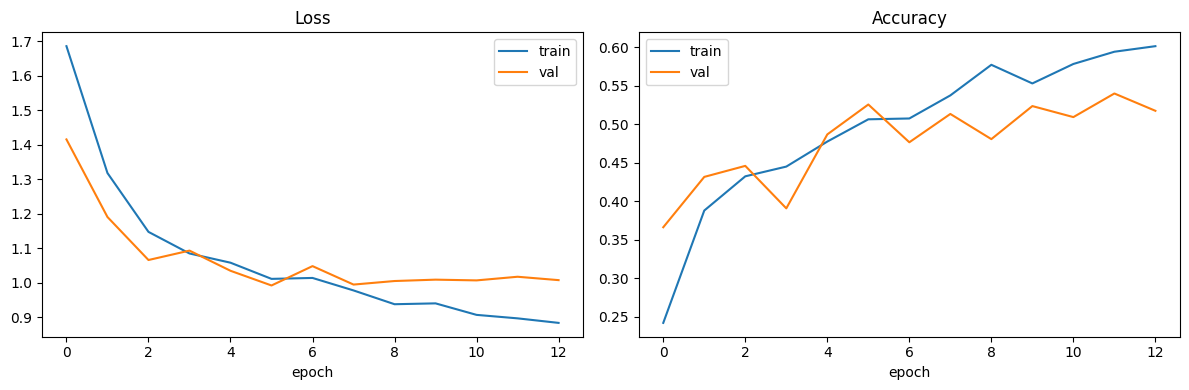
\includegraphics[width=\columnwidth]{training_curves.png}
  \caption{Baseline training. Left: cross-entropy loss; right: accuracy.
  Validation accuracy plateaus near $0.52$ while training accuracy keeps rising,
  i.e.\ the model overfits the single training set $S1$; early stopping halts
  training at epoch~13.}
  \label{fig:curves}
\end{figure}

\subsection{Contrastive extension: Supervised Contrastive Learning (F.~Vezzani)}
\label{sec:contrastive}
\emph{(Developed by F.~Vezzani; implemented and trained as Section~9 of the
notebook.)}

\subsubsection{Motivation}
The baseline is trained with plain cross-entropy on a single environment, so
nothing pushes its features to be invariant across domains. Following the
\emph{contrastive / self-supervised} direction suggested in the project
proposal, we implement \emph{Supervised Contrastive Learning}
(SupCon)~\cite{supcon}. The key change is \emph{what} is optimized: instead of
predicting the label directly, an \emph{encoder} is first trained so that two
windows of the \emph{same activity} are pulled together and windows of different
activities are pushed apart---\emph{regardless of the environment, person or
antenna they come from}. Because the objective depends only on activity
identity, the encoder is encouraged to discard environment-specific nuisances. A
tiny linear classifier is then fit on top of the frozen representation
(\emph{linear probe}).

\subsubsection{Domain-randomization augmentations}
SupCon needs, for each window, two augmented ``views'' that keep the activity
intact but perturb nuisance factors, acting as a light domain randomization
(\fig{fig:aug}). All transforms run on-GPU on a whole batch (default
parameters in parentheses):
\begin{itemize}
  \item \textbf{amplitude scaling} by a per-window random gain
  ($\mathcal{U}(0.8,1.2)$)---rooms/distances reflect the signal with different
  strength;
  \item \textbf{additive Gaussian noise} ($\sigma=0.05$);
  \item \textbf{circular time shift} ($\pm 40$ samples)---the activity does not
  depend on where in the $\approx 2$\,s window it starts;
  \item \textbf{time and Doppler masking} (SpecAugment-style: a zeroed band of
  $40$ time samples and $15$ velocity bins)---forces the encoder to use the whole
  time--velocity pattern rather than any single region.
\end{itemize}

\begin{figure}[t]
  \centering
  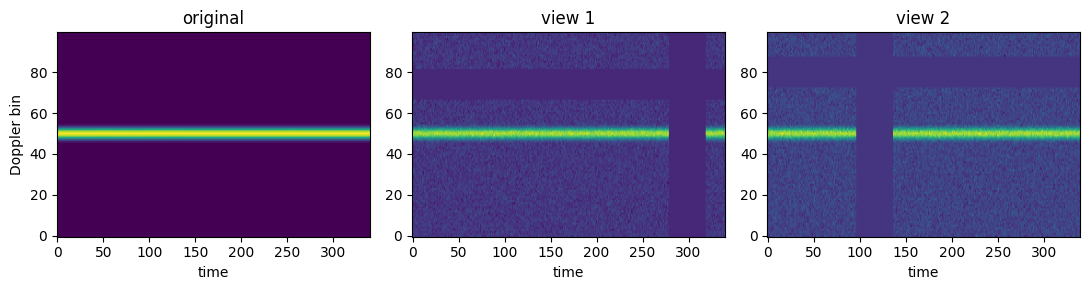
\includegraphics[width=\columnwidth]{augment_views.png}
  \caption{A window (\emph{left}) and two augmented views. Amplitude scaling and
  Gaussian noise change the texture; the circular time shift and the
  SpecAugment-style time/Doppler masks (dark bands) hide parts of the pattern,
  while the activity signature (the horizontal energy band) is preserved.}
  \label{fig:aug}
\end{figure}

\subsubsection{Encoder and projection head}
The encoder $f(\cdot)$ is a deeper, batch-normalized evolution of the baseline's
Inception block (\tab{tab:encoder}). It keeps the three-branch Inception
front-end (max-pool / strided conv / deeper conv, concatenated to $41$ channels)
but adds (i) batch normalization after every convolution, (ii) a $1\times1$
channel-mixing reduction to $32$ channels, (iii) a second downsampling stage
($32\!\rightarrow\!64\!\rightarrow\!128$), and (iv) \emph{global average
pooling}, replacing the baseline's large \texttt{flatten}$\rightarrow$dense layer
with a fixed $128$-dimensional representation $h$ that has fewer parameters and
is more shift-robust. A small MLP \emph{projection head} $g(\cdot)$
($128\!\rightarrow\!128\!\rightarrow\!128$, ReLU) maps $h$ to an
$L_2$-normalized embedding $\bm{z}=g(h)$ on the unit hypersphere; as prescribed by
SupCon, the loss is applied to $\bm{z}$ and the head is \emph{discarded} after
pre-training, so classification uses $h$. The whole model has $130{,}952$
parameters (encoder $\approx\!97.9$k $+$ head $\approx\!33$k), comparable to the
baseline's $128.5$k.

\begin{table}[t]
  \centering
  \caption{Contrastive encoder $f(\cdot)$; output sizes for a
  $1\times340\times100$ input. BN$+$ReLU follow every convolution; ``sN''
  denotes stride~N (default stride~1). The pooling output is the $128$-d
  representation $h$.}
  \label{tab:encoder}
  \setlength{\tabcolsep}{4pt}
  \begin{tabular}{@{}lll@{}}
    \toprule
    Stage & Layers & Output ($C\times H\times W$) \\
    \midrule
    Inception & maxpool(2); conv(16,s2); & $41\times170\times50$\\
              & conv(16)$\rightarrow$conv(24,s2) & \\
    Reduce    & conv(32,\,$1\times1$) & $32\times170\times50$\\
    Stage 2   & conv(64,s2)$\rightarrow$conv(128,s2) & $128\times43\times13$\\
    Pool      & global average pool & $128$\\
    \bottomrule
  \end{tabular}
\end{table}

\subsubsection{SupCon loss}
For a batch of $L_2$-normalized embeddings with labels, each anchor $i$ attracts
every other sample sharing its label (its positive set $P(i)$) and repels all
others, through a temperature-scaled softmax over cosine similarities:
\begin{equation}
\label{eq:supcon}
\mathcal{L}=\frac{1}{|I|}\sum_{i\in I}\frac{-1}{|P(i)|}\sum_{p\in P(i)}
\log\frac{\exp(\bm{z}_i\!\cdot\!\bm{z}_p/\tau)}
{\sum_{a\neq i}\exp(\bm{z}_i\!\cdot\!\bm{z}_a/\tau)},
\end{equation}
where $I$ is the set of anchors with at least one same-class positive (the
implementation averages the per-anchor terms over the batch) and the temperature
is $\tau=0.07$. Unlike self-supervised SimCLR~\cite{simclr}, using the labels in
\eq{eq:supcon} makes \emph{all} same-activity windows in the batch positives---even
those from different files or environments---which turns generic contrastive
learning into an environment-invariant \emph{activity} representation.

\subsubsection{Training and evaluation protocol}
Everything uses the \emph{same} $S1$-based split as the baseline.
\begin{itemize}
  \item \textbf{Contrastive pre-training.} Each batch is expanded into two
  augmented views; encoder and head are trained jointly with Adam
  (lr~$10^{-3}$, weight decay~$10^{-4}$) for up to $30$ epochs with early
  stopping (patience~$7$) on the validation contrastive loss, keeping the best
  encoder.
  \item \textbf{Linear probe.} The encoder is frozen, embeddings are
  pre-computed and standardized with training statistics, and a single
  $\mathrm{Linear}(128,5)$ layer is trained with cross-entropy (Adam,
  lr~$10^{-3}$, early stopping). This isolates the quality of the representation.
  \item \textbf{Optional fine-tuning.} The encoder is then unfrozen and the full
  network fine-tuned end-to-end with a small learning rate ($10^{-4}$).
\end{itemize}
The model is evaluated under the same cross-domain protocol as the baseline
(train on $S1$, test on $S2$--$S7$). A t-SNE projection of the test embeddings,
colored by activity and by environment, is used as a diagnostic of
environment-invariance.
